\include{common_start}
\include{tutBlatt_methods}
\include{amsmath}

\tutnr{11}

\section{Rückblick}
\subsection{Rückblick}

\begin{frame}
	\frametitle{Rückblick}
	Was bisher geschah...

\end{frame}


\section{Multiple Choice}
\subsection{Multiple Choice}
\begin{frame}
	\frametitle{Multiple Choice}
	\begin{center}
	\only<1>{
		Das Hamilton-Kreis Problem ist NP-vollständig
	}
	\only<2>{
		In der Klasse NP liegen nicht-entscheidbare Probleme
	}
	\only<3>{
		Das Vertex-Cover Problem ist NP-vollständig
	}
	\only<4>{
		Semi-entscheidbare Sprachen sind unter Komplementbildung
abgeschlossen
	}
	\only<5>{
		Nichtdeterministische endliche Automaten sind echt mächtiger als
deterministische
	}
	\only<6>{
		Zu jeder CH-2-Sprache gibt es eine CH-1-Grammatik
	}
	\only<7>{
		Um zu zeigen, dass ein Problem $\Pi$ NP-vollständig ist, genügt es, ein NP-schweres Problem auf $\Pi$ zu reduzieren.
	}
	\end{center}
\end{frame}

\section{Neuanfang}
\subsection{Neuanfang}

\begin{frame}
	\frametitle{Neuanfang}
	Informationstheorie

\end{frame}

\section{Kolmogorov Komplexität}
\subsection{Kolmogorov Komplexität}

\section{Kolmogorow Komplexität}
\subsection{Kolmogorow Komplexität erklären}

\begin{frame}
	\frametitle{Kolmogorow}
	\only<1>{Beispiel: Das Wort, das aus 1000 Nullen besteht (Alphabet: ASCII)~\\~\\}
	\only<2>{00000000000000000000000000000000000000000000000000~\\
	00000000000000000000000000000000000000000000000000~\\
	00000000000000000000000000000000000000000000000000~\\
	00000000000000000000000000000000000000000000000000~\\
	00000000000000000000000000000000000000000000000000~\\
	00000000000000000000000000000000000000000000000000~\\
	00000000000000000000000000000000000000000000000000~\\
	00000000000000000000000000000000000000000000000000~\\
	00000000000000000000000000000000000000000000000000~\\
	00000000000000000000000000000000000000000000000000~\\
	00000000000000000000000000000000000000000000000000~\\
	00000000000000000000000000000000000000000000000000~\\
	00000000000000000000000000000000000000000000000000~\\
	00000000000000000000000000000000000000000000000000~\\
	00000000000000000000000000000000000000000000000000~\\
	00000000000000000000000000000000000000000000000000}
	\only<3>{Eine Beschreibung eines Wortes w ist ein Programm bei dessen Ausführung das Wort erzeugt wird. Die Länge dieses Programmes ist dann ein d(w).~\\~\\
	Program Nullfolge (n)~\\
	"" begin~\\
	"" "" for i:= 1 to n ~\\
    "" "" "" print ``0''~\\
	"" end}
\end{frame}

\begin{frame}
	\frametitle{Kolmogorow}
	Eine minimale Beschreibung eines Wortes $w$ heißt Kolmogorow-Komplexität $K(w)$
	\begin{itemize}
		\item Also: $\forall d(w): |d(w)| \geq |K(w)|$
		\item Die Länge von $K(w)$ ist abhängig von der Struktur von $w$
	\end{itemize}~\\
	Falls $|K(w)| \geq |w|$ heißt das Wort unkomprimierbar.~\\~\\
	Die Kolmogorow-Komplexität ist nicht \only<1>{entscheidbar}\only<2>{berechenbar} aber \only<1>{semi-entscheidbar}\only<2>{rekursiv aufzählbar}.

\end{frame}

\subsection{Kolmogorow Aufgabe}
\begin{frame}
	\frametitle{Kolmogorow Komplexität: Aufgabe (B7 A1)}
	\begin{enumerate}
		\item Beweisen Sie, dass $K(x)$ nicht berechenbar ist!
		\item Beweisen Sie, dass die Menge der nichtkomprimierbaren Strings $\mathcal{L}$
		nicht rekursiv aufz"ahlbar ist!
		\item Geben Sie eine m"oglichst gute obere Schranke f"ur die Kolmogorow-Komplexit"at von $0^n$ an!
		\item Geben Sie eine m"oglichst gute obere Schranke f"ur die Kolmogorow-Komplexit"at der
		Bin"ardarstellung der $n$-ten\\ Primzahl $p$ an!
		\item Sei $x$ ein Palindrom. Geben sie eine m"oglichst gute obere Schranke f"ur $K(x)$ an!
		\item Sei $\pi_n$ die Kreiszahl $\pi$ bis zur $n$-ten Nachkommastelle entwickelt. Geben Sie eine m"oglichst gute obere Schranke f"ur $\pi_n$ an.
	\end{enumerate}
\end{frame}

\begin{frame}
	\frametitle{Kolmogorov Komplexität}
		\textbf{Vorsicht:} Aufpassen, in Abhängigkeit wovon eine obere Schranke angegeben werden soll.
	
\end{frame}
\begin{frame}
\begin{center}
\vspace{-0.3cm}
	\includegraphics[height=0.9\textheight]{images/Mandelpart2_red.png}
\end{center}
\end{frame}

\section{Begriffe der Informationstheorie}
\subsection{Erklärung}
\begin{frame}
	\frametitle{Shannonscher Informationsbegriff}
	\begin{itemize}
		\item Jede Information bzw. Nachricht besitzt eine Quelle
		\begin{itemize}
			\item Oft randomisiert a.k.a. Zufallsquellen
			\item Wenn alle gesendete Nachrichten unabhängig voneinander sind, ist die Quelle gedächtnislos
		\end{itemize}
		\item Es gibt immer einen Empfänger, der die Nachrichten beobachtet
		\item Je unvorhersehbarer die Nachricht, desto mehr Informationsgehalt
		\begin{itemize}
				\item Wird deshalb auch manchmal Überraschungswert genannt
		\end{itemize}
		\item Entropie ist ein Begriff für die Dichte der Informationen
	\end{itemize}
\end{frame}

\begin{frame}
	\frametitle{Etwas genauer}
	\begin{itemize}
		\item Informationsgehalt soll nicht negativ sein
		\item Ein sicheres Ergebnis (p = 1) enthält keine Information
		\item Informationen von unabhängigen Nachrichten sollen sich addieren
		\item Kleine Änderungen der Wahrscheinlichkeit $\Rightarrow$ kleine Änderung des Informationsgehalts
		\item $I(x) = -log_b(p(x)) = log_b(\frac{1}{p(x)})$ erfüllt diese Bedingungen
		\begin{itemize}
			\item Meist wird als Basis b = 2 verwendet
		\end{itemize}~\\~\\
		\item Entropie ist entsprechend definiert~\\ $H(X) = \sum\limits_{x \in X} (p(x) \cdot log_2(\frac{1}{p(x)})) = \sum\limits_{x \in X} (p(x) \cdot I(x))$
	\end{itemize}
\end{frame}

\begin{frame}
	\frametitle{Beispiele}
	\begin{itemize}
		\item Zufallsquelle 1: p(A) = $\frac{1}{2}$, p(B) = $\frac{1}{2}$
		\item I(A) = $log_2(\frac{1}{0.5}) = log_2(2) = 1$ = I(B)
		\item H(X) = $(p(A) \cdot I(A)) + (p(B) \cdot I(B)) = 0.5 + 0.5 = 1$~\\~\\~\\~\\
		\item Zufallsquelle 2: p(A) = $\frac{1}{16}$, p(B) = $\frac{15}{16}$
		\item I(A) = $log_2(\frac{1}{0.0625}) = log_2(16) = 4$
		\item I(B) = $log_2(\frac{1}{0.9375}) = log_2(\frac{16}{15}) = 0.0931\ldots$
		\item H(X) = $(p(A) \cdot I(A)) + (p(B) \cdot I(B))$~\\$= (\frac{1}{16} \cdot 4) + (\frac{15}{16} \cdot 0.0931) = \frac{1}{4} + 0.873 = 0.337$
	\end{itemize}
\end{frame}
%Explaining "Ordnung von Zeichenketten would be Bogus"

\subsection{Aufgabe B11 A1}
\begin{frame}
	\frametitle{Aufgabe B11 A1}
	\begin{enumerate}
		\item Wie gro"s sind der Informationsgehalt und die Entropie, wenn eine Quelle mit
		dem Alphabet $\{0,1\}$ nur aus dem Zeichen $0$ bestehende Folgen sendet?
		\item An einer Quelle mit $n$ Zeichen tritt jedes Zeichen gleichverteilt auf. Wie
		gro"s sind der Informationsgehalt und die Entropie eines einzelnen Zeichens?
		\item Berechnen Sie die Entropie des Wurfes eines idealen W"urfels mit 8 Seiten,
		dessen Wahrscheinlichkeit f"ur jede Seite $p = \frac{1}{8}$ ist!
		\item Was ist der Unterschied zwischen den beiden Folgen, die aus verschiedenen
		ged"achtnislosen Quellen mit der gleichen Wahrscheinlichkeit f"ur $0$ und $1$
		gesendet werden, wenn man sie unter dem Aspekt Entropie und Ordnung betrachtet?
		\begin{enumerate}
			\item ...10101010101010101010...
			\item ...01101100110111000010...
		\end{enumerate}
	\end{enumerate}
\end{frame}

\section{Mehr Begriffe der Informationstheorie}
%Erklären: Empfänger, Kanäle, Verbundentropie, Äquivokation, Transinformation, Fehlinformation(="inverse Äquivokation"=Irrelevanz?), Totalinformation (=Verbundentropie?)
\begin{frame}
\frametitle{Übertragung von Information}
Daten können über einen Kanal von der Quelle zu einem Empfänger gesendet werden. Dieser Kanal ist in der Regel nicht störungsfrei, dass heißt die gesendeten Daten können ungleich zu den empfangenen sein.\\ 
Ein gestörter Kanal kann durch seine Übertragungswahrscheinlichkeiten $P(r|q)$, welche angeben wie wahrscheinlich es ist, dass r beim Empfänger ankommt, wenn q aus der Quelle gesendet wurde, charakterisiert werden.\\
Damit ergibt sich der Zusammenhang \[P(R=r)=\sum_{q \in Q} P(Q=q)P(R=r|Q=q)\] und für die Wahrscheinlichkeit das r und q gleichzeitig auftreten: \[P(Q=q,R=r)=P(Q=q)P(R=r|Q=q).\]
\end{frame}
\begin{frame}
\frametitle{Einige Definitionen}
\emph{Totalinformation} oder auch Verbundentropie H(Quelle $Q$, Empfänger $R$) ist die gesamte von Quelle und Empfänger erzeugte Entropie
\[H(Q,R)=-\sum_{q \in Q} \sum_{r \in R} P(Q=q,R=r)\log(P(Q=q,R=r))\]
\emph{Äquivokation} $H$(Quelle $Q|$ Empfänger $R$) gibt dem Entropieverlust durch die Übertragung an.\\
\[H(Q|R)=H(Q,R)-H(R)\]
\emph{Fehlinformation} H(Empfänger $R|$ Quelle $Q$) entspricht dem anscheinenden Entropiegewinn durch die Übertragung.
\[H(R|Q)=H(Q,R)-H(Q)\]
\emph{Transinformation} I(Quelle $Q$, Empfänger $R$) ist die richtig empfangene Informationsmenge.
\[I(Q,R)= H(Q)-H(Q|R)=H(R)-H(R|Q)=H(Q)+H(R)-H(Q,R)\]
\end{frame}
\begin{frame}
\frametitle{Bild zur Veranschaulichung}
\begin{center}
\includegraphics[scale=0.35]{images/Entropie_XY}
\end{center}
\end{frame}
\subsection{Erklärung}
\subsection{Aufgabe B11 A2}
\begin{frame}
	\frametitle{Aufgabe B11 A2}
	\only<1>{
	Studieren Sie den Fall eines asymmetrischen bin"aren Kanals mit Quelle $X$ und
	Empf"anger $Y$. Die "Ubertragungswahrscheinlichkeiten $P(Y|X)$ seien durch das
	folgende Diagramm gegeben:
	}
	\only<2->{
	\vspace{-0.6cm}
	}
		\begin{center}
			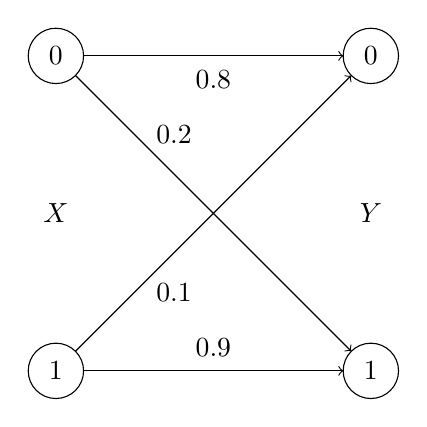
\begin{tikzpicture}
			\draw (0,0) circle (10pt);
			\draw (0,0) node {$1$};
			\draw (0,2) node {$X$};
			\draw (0,4) circle (10pt);
			\draw (0,4) node {$0$};
			\draw (4,0) circle (10pt);
			\draw (4,0) node {$1$};
			\draw (4,2) node {$Y$};
			\draw (4,4) circle (10pt);
			\draw (4,4) node {$0$};
			\draw [->] (0.35,0) -- (3.65,0);
			\draw (2,0.3) node {$0.9$};
			\draw [->] (0.35,4) -- (3.65,4);
			\draw (2,3.7) node {$0.8$};
			\draw [->] (0.25,0.25) -- (3.75,3.75);
			\draw (1.5,1) node {$0.1$};
			\draw [->] (0.25,3.75) -- (3.75,0.25);
			\draw (1.5,3) node {$0.2$};
			\end{tikzpicture}
		\end{center}
		\only<2,3>{
	\begin{enumerate}
		\only<2>{
		\item Wie gro"s ist die Wahrscheinlichkeit daf"ur, dass die Bitkette ``$1100$'' als
		``$1001$'' "ubertragen wird?
		\item Wenn die Entropie der Quelle $H(X) = 1 \; \mbox{bit}$ ist, wie gro"s ist dann
		$H(Y)$?
		\item Wie gro"s muss $H(X)$ sein, damit $H(Y) = 1 \; \mbox{bit}$ gilt?
		}
		\only<3>{
		\item Wie gro"s ist die Verbundentropie $H(X,Y)$ des "Ubertragungssystems? Gehen Sie
		ab dieser Teilaufgabe von der Situation der 2. Teilaufgabe aus!
		\item Wie gro"s ist die sog. Irrelevanz $H(Y|X)$? Und wie gro"s ist die sog.
		"Aquivokation $H(X|Y)$?
		\item Wie gro"s ist schlie"slich die Transinformation $I(X;Y)$?	
	}
	\end{enumerate}
	}
\end{frame}
\subsection{Aufgabe B11 A4}
\begin{frame}
	\frametitle{Aufgabe B11 A4}
	Gegeben sei eine ged"achtnislose Quelle $Q$, die mit Wahrscheinlichkeit $p_0 =
	\frac{1}{4}$ eine $0$ und mit Wahrscheinlichkeit $p_1 = \frac{3}{4}$ eine $1$ sendet.
	Gegeben sei zudem ein Empf"anger $R$, der die Zeichen von $Q$ zu empfangen versucht.
	Dieser Empf"anger empf"angt eine $0$ immer richtig. Sendet die Quelle $Q$ jedoch
	eine $1$, so empf"angt $R$ mit Wahrscheinlichkeit $\frac{1}{2}$ eine $1$ und mit
	Wahrscheinlichkeit $\frac{1}{2}$ eine $0$.
	\begin{enumerate}
		\item Berechnen Sie die Information $I(0)$ und $I(1)$ bez"uglich der Quelle $Q$!
		\item Berechnen Sie die Entropie der Quelle $Q$!
		\item Die Quelle $Q$ sendet die Zeichenfolge $0110$. Wie hoch ist der
		Informationsgehalt dieser Zeichenfolge?
		\item Berechnen Sie die Totalinformation $H(Q,R)$, die Fehlinformation $H(R|Q)$,
		die "Aquivokation $H(Q|R)$ und die Transinformation $I(Q;R)$!
	\end{enumerate}
\end{frame}

\section{Schluss}
\subsection{Schluss}
\begin{frame}
\frametitle{Bis zum nächsten Mal!}
	\center{Kolmogorov Directions}
\begin{center}
	\includegraphics[height=0.85\textheight]{images/kolmogorov_directions.png}
\end{center}
\end{frame}

\include{common_end}